\subsection{Privacy of the complete transcript}\label{sec:privacy}
The following statements concern the specified ideal kernels under
Section~\ref{sec:assumptions}. They are not a certification of every floating-point
instruction in the simulator.

\begin{proposition}[REM on a common road domain]\label{prop:rem}
For any nonempty finite common $V$, (\ref{eq:rem}) is $u$-Geo-I.
Mapping the sampled road state to its coordinate preserves the bound.
\end{proposition}
\begin{proof}
Let $d=\|x-x'\|_2$, $w_x(v)=\exp[-u\|x-a_v\|_2/2]$ and
$S_x=\sum_vw_x(v)$. The reverse triangle inequality bounds
$w_x(v)/w_{x'}(v)$ by $e^{ud/2}$. Summing
$w_{x'}(v)\le e^{ud/2}w_x(v)$ over the same domain bounds $S_{x'}/S_x$
by the same factor. Their product gives $R_u(v\mid x)/R_u(v\mid x')\le e^{ud}$.
Summation proves the event bound, including coordinate aliases.
\end{proof}

\begin{proposition}[Private tests and session accounting]\label{prop:history}
Under prospective accounting, the protected history $E$ obeys
\begin{equation}
\Pr_X(E\in B)\le e^{C_sD_\infty(X,X')}\Pr_{X'}(E\in B). \label{eq:history}
\end{equation}
\end{proposition}
\begin{proof}
At a fixed protected history, $h$ is fixed and $x\mapsto\|x-h\|_2$ is
1-Lipschitz. The Laplace density ratio of the noisy distance is at most
$e^{u\|x-x'\|_2}$, so either threshold event costs one unit.
The extended reuse branch has probability $r_x$; refresh-and-state has
probability $(1-r_x)R_u(v\mid x)$. Its ratio costs at most two units.
The first reference costs one. At each common prefix the filter makes its
read decision before private access. Chain rule bounds the log ratio of any
extended history by $u\sum_i c_i\|x_i-x_i'\|_2\le C_sD_\infty$.
Marginalizing the flags and summing over the event proves (\ref{eq:history}).
No independence between successive GPS positions is assumed.
\end{proof}

\begin{proposition}[One bounded segment]\label{prop:kernel}
With common positive $w$, scores in $[0,1]$ and
$\alpha=\varepsilon/(2+\varepsilon)$, (\ref{eq:kernel}) is a positive PMF and
$p_a(b)/p_a(b')\le1+\varepsilon$ for every pair of beliefs.
\end{proposition}
\begin{proof}
Centering gives $\sum_ap_a=1$. Since $z_a-\mu\in[-1,1]$,
$w_a(1-\alpha)\le p_a\le w_a(1+\alpha)$. Dividing yields
$(1+\alpha)/(1-\alpha)=1+\varepsilon$. Conditional mixtures over random
beliefs remain in the same interval. For (\ref{eq:integer}), summing weights
cancels the centered term and yields total $DT^2S$; the normalized weight is
exactly $p_a$.
\end{proof}

\begin{proposition}[Adaptive segment composition]\label{prop:segments}
Under the common-prefix and publication assumptions, the entire ordered wire satisfies
\begin{equation}
\Pr_X(O_n\in B)\le R_n\Pr_{X'}(O_n\in B),\qquad
R_n=\prod_{j=1}^n(1+\varepsilon_{Q,j})\le e^{\Gamma_Q}. \label{eq:segments}
\end{equation}
\end{proposition}
\begin{proof}
Condition on augmented history, including fake lane states. Each action ratio is bounded
by Proposition~\ref{prop:kernel}. Provider responses have the same conditional law;
committed frames and fixed retries are post-processing. Chain rule multiplies the
action factors, and projection removes augmented state. Finally,
$\sum_{j=1}^n\varepsilon_{Q,j}=\Gamma_Q n/(n+1)$ and $1+t\le e^t$.
This argument uses conditional laws, not independent segments.
\end{proof}

The bound holds for every prefix without a known duration. For $\Gamma_Q=1$, a
rational certificate gives $R_\infty<2.437372$. Specifically,
$P_N=\prod_{j\le N}(1+1/[j(j+1)])$ and the tail sum is $1/(N+1)$.
Bounding elementary symmetric tail sums by powers of that sum yields
$R_\infty\le P_N/[1-1/(N+1)]$; $N=11$ already gives the stated outward-rounded
ceiling. The uniform cylinder-event bound also extends to an infinite transcript
under the same channel model. As $j$ grows, $\alpha_j$ vanishes and adaptation
approaches the public base; finite disclosure does not promise indefinitely
strong tracking of new GPS.

\begin{theorem}[Conditional end-to-end guarantee]\label{thm:endtoend}
If downstream uses only protected history and permitted context, and both the
spatial and Q assumptions hold, then
\begin{equation}
\Pr_X(O_n\in B)\le
\exp\!\bigl(\min\{C_sD_\infty(X,X'),\log R_n\}\bigr)
\Pr_{X'}(O_n\in B). \label{eq:endtoend}
\end{equation}
\end{theorem}
\begin{proof}
The common downstream kernel integrates the protected-history inequality
(\ref{eq:history}), giving its post-processing bound. Proposition~\ref{prop:segments}
independently bounds the same wire event. Taking the smaller ceiling proves the
claim. The two budgets are not added: $C_s$ has units $\mathrm m^{-1}$,
whereas the Q allowance is dimensionless.
\end{proof}

The Q bound can remain valid without an ideal upstream Geo-I implementation,
provided its own assumptions hold. The spatial branch requires the upstream
conditions. With the current parameters, the coarse spatial envelope crosses the
all-duration Q ceiling at $\log(2.437372)/0.23\approx3.874$ m; beyond that
distance the Q envelope is smaller. Hence strong quantitative transcript protection
must not be attributed to Geo-I alone.

\begin{figure}[htbp]\centering
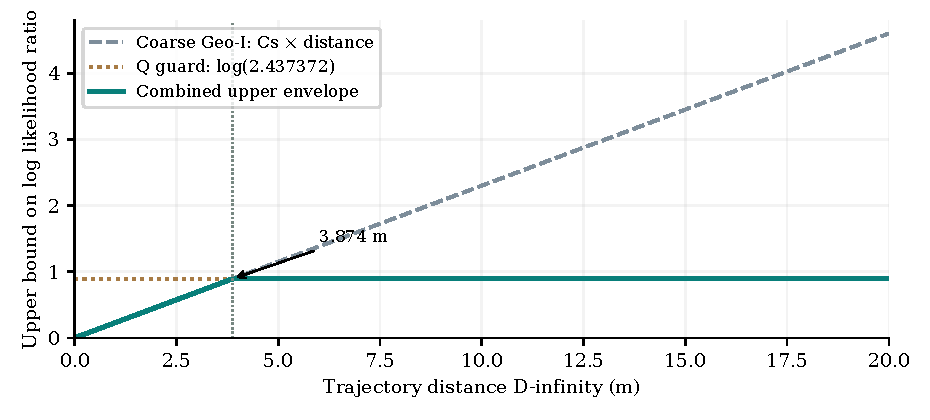
\includegraphics[width=.86\linewidth]{figure_bound_profile.pdf}
\caption{Illustrative upper envelopes for the frozen parameters, not an
empirical privacy curve. The minimum uses both sets of assumptions.
The spatial term is coarse; the dimensionless Q guard dominates beyond
approximately 3.874 m.}\label{fig:bound-profile}
\end{figure}

\begin{corollary}[Arbitrary-estimator localization]\label{cor:hit}
At the same context $C$, suppose the Q ratio bound $R$ holds uniformly over the
support of a valid trajectory prior. Define
$\pi_{\max,t}(r)=\sup_y\Pr(\|X_t-y\|_2\le r\mid C)$. Every measurable estimator
$\widehat x_t(O)$ satisfies
\begin{equation}
\Pr(\|X_t-\widehat x_t(O)\|_2\le r\mid C)
\le \frac{R\pi_{\max,t}(r)}{1+(R-1)\pi_{\max,t}(r)}. \label{eq:hit}
\end{equation}
\end{corollary}
\begin{proof}
For a realized output $o$, fix the private-input event inside the radius-$r$
ball centered at $\widehat x_t(o)$. Mixture likelihood ratios give the posterior-odds
ceiling $f_R(\pi)=R\pi/[1+(R-1)\pi]$ for that event. Its prior is at most
$\pi_{\max,t}(r)$, and $f_R$ is increasing. Integrating over outputs proves the
claim. Weighted time averages follow by linearity without independent errors.
Finite/countable outputs, or an appropriate common-density version, are understood.
\end{proof}
Choosing $r=100$ m links the theorem to Hit100, but does not infer its empirical
value from the theorem. A strong spatial prior can make the bound uninformative.
In a balanced binary illustration, the one-session ceiling corresponds to posterior
at most approximately 70.91\%, not to an asserted average attack accuracy.

\begin{corollary}[Conditional joint channels]\label{cor:joint}
If each of $m$ channels has a conditional ratio bound $R_\ell$ at every feasible
common joint prefix, their joint transcript has ratio at most $\prod_\ell R_\ell$.
Private inputs may be correlated.
\end{corollary}
Chain rule proves the statement; marginal per-channel guarantees alone are not its
assumption. Two valid $\Gamma_Q=1$ channels give a balanced-prior posterior ceiling
below 85.5925\%, rather than the one-session 70.91\%. A Raw partner lacks the required
finite guard. Likewise, $\Gamma_Q=0$ yields $p=w$ at every prefix, so its wire law is
independent of the private trajectory at fixed context under the public-channel
assumptions. Positive adaptation is a permitted design choice, not a privacy necessity.

\subsection{Utility properties and their scope}\label{sec:utility}
At the same local state, let $r_a\in[0,1]$ denote actual conditional utility of action
$a$. Centering gives, for any vector $f$,
$\E_pf-\E_wf=\alpha\Cov_w(z,f)$. In particular,
\begin{align}
\E_pz-\E_wz&=\alpha\Var_w(z)\ge0,\\
\E_pr-\E_wr&=\alpha\Cov_w(z,r). \label{eq:gain}
\end{align}
For a proxy $v$ satisfying $\max_a|r_a-v_a|\le\eta$,
\begin{equation}
\E_pr-\E_wr\ge\alpha\{\Cov_w(z,v)-\eta\E_w|z-\E_wz|\}. \label{eq:calibration}
\end{equation}
The uncertainty in $\eta$ cannot be set to zero because belief uses Bayes' rule.
The nonnegative score gain is not a nonnegative actual Recall gain.

Let $T_t$ be the full-catalogue reference top-$k$ after filtering and deterministic
tie-breaking, and $U_t$ the valid received metadata. Local top-$k$, used for evaluation
only, obeys
\begin{equation}
\operatorname{Recall@}k=\frac{|T_t\cap U_t|}{|T_t|},\qquad T_t\ne\varnothing. \label{eq:recall}
\end{equation}
Every received reference item precedes every non-reference item in the same order.
Thus it survives local top-$k$, proving (\ref{eq:recall}). Set inclusion of valid
caches cannot reduce Recall at the same GPS/request. It does not imply monotone
Recall while GPS or requests change, nor does ranking create missing metadata.

For a whole-session comparison, let $P_n$ be the adaptive history law and $W_n$ the
\emph{identical} public policy with $\Gamma_Q=0$, including the same provider and
external conditions. At each fixed prefix,
$\chi^2(p_j\Vert w_j)=\alpha_j^2\Var_{w_j}(z_j)\le\alpha_j^2/4$.
If the protected score remains latent at that prefix, $z_j$ here denotes its
conditional mean under the adaptive law; it is still bounded in $[0,1]$.
A conditional second-moment recursion then yields, for every $h\in[0,1]$,
\begin{align}
|\E_{P_n}h-\E_{W_n}h|
&\le\TV(P_n,W_n)\\
&\le\frac12\sqrt{\prod_{j\le n}(1+\alpha_j^2/4)-1}. \label{eq:tv}
\end{align}
For $\Gamma_Q=1$, a rational tail certificate gives a uniform ceiling below
0.0553. This bounds a possible difference from a matched base, not absolute
utility or superiority to another paper. The sign remains empirical.

Finally, at a fixed history, let $\rho$ be a declared public case law and $\lambda$
the actual case law. If $\E_\rho\widehat r\ge c$,
$\TV(\lambda,\rho)\le\tau$ and $\E_\lambda|r-\widehat r|\le\nu$, then
\begin{equation}
\E_\lambda r\ge\max\{0,c-\tau-\nu\}. \label{eq:floor}
\end{equation}
Conditional expectation and public time weights extend this to a session without
IID assumptions. The supplement gives exact nonvacuous finite examples and a
negative actual-gain counterexample. Real-provider calibration is not certified
by these illustrations.

Purpose-independent payloads supply a separate interface property: changing $\psi$
at fixed trajectory, context and randomness does not change the cover request.
This conditional noninterference does not remove intent correlated with location.
The complete practical guarantee still depends on state persistence, entropy,
numerical support and absence of additional side channels. Floating-point privacy
implementations require care~\cite{mironov}; our ideal analysis and integer Q
representation are not a complete deployment certificate.
